% $Header$

\documentclass{beamer}
\usefonttheme[onlymath]{serif}
\newcommand\bmale{\fontsize{6}{7.2}\selectfont}
\newcommand\male{\fontsize{8}{7.2}\selectfont}
\newcommand\normalne{\fontsize{10}{7.2}\selectfont}
\newcommand\duze{\fontsize{12}{7.2}\selectfont}
% This file is a solution template for:

% - Talk at a conference/colloquium.
% - Talk length is about 20min.
% - Style is ornate.



% Copyright 2004 by Till Tantau <tantau@users.sourceforge.net>.
%
% In principle, this file can be redistributed and/or modified under
% the terms of the GNU Public License, version 2.
%
% However, this file is supposed to be a template to be modified
% for your own needs. For this reason, if you use this file as a
% template and not specifically distribute it as part of a another
% package/program, I grant the extra permission to freely copy and
% modify this file as you see fit and even to delete this copyright
% notice. 


\mode<presentation>
{
  \usetheme{CambridgeUS}
  \usecolortheme{beaver}
  % or ...

  %\setbeamercovered{transparent}
  % or whatever (possibly just delete it)
}

\usepackage{ulem}
\usepackage[T1]{fontenc}
\usepackage[polish]{babel}
\usepackage[utf8]{inputenc}
\selectlanguage{polish}
\usepackage{tabto}
% or whatever

%\usepackage[latin1]{inputenc}
%% or whatever

\usepackage{lmodern}
\usepackage[T1]{fontenc}
% Or whatever. Note that the encoding and the font should match. If T1
% does not look nice, try deleting the line with the fontenc.


\title[Analizy mikrosymulacyjne] % (optional, use only with long paper titles)
{Analizy mikrosymulacyjne - wykłady}

\subtitle
{Ruch i jego reprezentacja}

\author[dr inż. Rafał Kucharski] % (optional, use only with lots of authors)
{dr inż. Rafał~Kucharski\inst{1}}
% - Give the names in the same order as the appear in the paper.
% - Use the \inst{?} command only if the authors have different
%   affiliation.

\institute[] % (optional, but mostly needed)
{
  \inst{1}%
  Zakład Systemów Komunikacyjnych\\
  Politechnika Krakowska
  \and
 }
% - Use the \inst command only if there are several affiliations.
% - Keep it simple, no one is interested in your street address.

\date[ZSK, L-2, WIL, PK] % (optional, should be abbreviation of conference name)
{Kraków, 2017}
% - Either use conference name or its abbreviation.
% - Not really informative to the audience, more for people (including
%   yourself) who are reading the slides online



% If you have a file called "university-logo-filename.xxx", where xxx
% is a graphic format that can be processed by latex or pdflatex,
% resp., then you can add a logo as follows:

\pgfdeclareimage[height=1cm]{university-logo}{ZSK}
 \logo{\pgfuseimage{university-logo}}

% Delete this, if you do not want the table of contents to pop up at
% the beginning of each subsection:
\AtBeginSubsection[]
%{
%  \begin{frame}<beamer>{Outline}
%    \tableofcontents[currentsection,currentsubsection]
%  \end{frame}
%}


% If you wish to uncover everything in a step-wise fashion, uncomment
% the following command: 

%\beamerdefaultoverlayspecification{<+->}


\begin{document}

\begin{frame}
  \titlepage
\end{frame}

%\begin{frame}{Zakres}
%  \tableofcontents
%  % You might wish to add the option [pausesections]
%\end{frame}


% Structuring a talk is a difficult task and the following structure
% may not be suitable. Here are some rules that apply for this
% solution: 

% - Exactly two or three sections (other than the summary).
% - At *most* three subsections per section.
% - Talk about 30s to 2min per frame. So there should be between about
%   15 and 30 frames, all told.

% - A conference audience is likely to know very little of what you
%   are going to talk about. So *simplify*!
% - In a 20min talk, getting the main ideas across is hard
%   enough. Leave out details, even if it means being less precise than
%   you think necessary.
% - If you omit details that are vital to the proof/implementation,
%   just say so once. Everybody will be happy with that.

\section{Wykład 1}

\subsection{Sprawy organizacyjne}

\begin{frame}{Sprawy formalne}
 
  \begin{itemize}
  \item cztery wykłady
  \item esencja
  \item obecność wysoce wskazana
  \item treść wykładów wymagana do zaliczenia 
  \end{itemize}
\end{frame}

\begin{frame}{Terminy wykładów}
 sala 404 WIL \\  godzina 16:15 
   \begin{itemize}
  \item 09.05.2017
  \item 23.05.2017
  \item 30.05.2017
  \item \sout{06.06.2017}
  \item 13.06.2017
  \end{itemize}
  
\end{frame}


\begin{frame}{Zakres wykładów}


\begin{itemize}
\item opis ruchu drogowego, miary ruchu i ich pomiary
\item dynamika ruchu
\item mikro, a makro skala
\item od opisu ogólnego do szczegółowego:
\begin{itemize}
\item markoskopowa funkcja oporu $\longrightarrow$ diagram fundamentalny \\ $\longrightarrow$ wykres: czas-przestrzeń-prędkość $\longrightarrow$ mikrosymulacja
\end{itemize}
\item modele mikroskopowe: 
\begin{itemize}
\item modele podążania za liderem:
\begin{itemize}
\item modele analityczne (optymalne), 
\item modele rzeczywiste (\textit{np. Intelligent Driver Model, Wiedemann’a}) 
\end{itemize}
\item modele dyskretne (zmiana pasa, decyzja o włączeniu się)
\end{itemize}
\item losowość (niedeterministyczność) w podejściu symulacyjnym
\item mikrosymulacja transportu zbiorowego
 \end{itemize}
\end{frame}

\begin{frame}{Literatura}

\begin{itemize}
\bmale
\item Treiber, M.,  Kesting, A. (2013). Traffic flow dynamics: Data, Models and Simulation. \footnote{\bmale większość grafik w wykładach pochodzi z tej książki}
\item Vissim - User Manual 
\item Newell, G. F. (2002). A simplified car-following theory: a lower order model. 
\item Daganzo, C. F. (1995). Requiem for second-order fluid approximations of traffic flow. 
\item Viti, F.,  van Zuylen, H. (2004). Modeling queues at signalized intersections.
\item Cats, O., \dots (2010). Mesoscopic simulation for transit operations. 
\item Kesting, A., Treiber, M., Helbing, D. (2010). Enhanced intelligent driver model to access the impact of driving strategies on traffic capacity. 
\item Gentile, G. (2010). The General Link Transmission Model for dynamic network loading and a comparison with the DUE algorithm
\item Kucharski, R., Drabicki, A. (2017). Estimating Macroscopic Volume Delay Functions with the Traffic Density Derived from Measured Speeds and Flows. 
\item Kucharski, R., Drabicki, A., Szarata, A. (2016). Modelowanie oporu skrzyżowań w modelach makroskopowych. Transport Miejski i Regionalny, (8), 14-19.
\item Tiddi, D., Kostic, B., Gentile, G. (2013). Conflict Areas for Macroscopic Models in Dynamic Traffic Assignment. 
\end{itemize}
\end{frame}


\subsection{Ruch i jego reprezentacja}

\label{2.1}
\begin{frame}{Ruch drogowy}{zapis faktycznych zjawisk}
Zapis dla:
\begin{itemize}
\item odcinków \\ \bmale \url{https://www.youtube.com/watch?v=MtwY9xKfaYo}{} \normalne
\item skrzyżowań\\ \bmale \url{https://www.youtube.com/watch?v=FF7ByafPOOk}{} \normalne
\end{itemize}
Ruch jest:
\begin{itemize}
\item złożony
\item zmienny (losowy)
\item ludzki, nie analityczny
\item ale jednak jest w nim pewna regularność, która można opisać analitycznie (fizycznie).
\end{itemize}
\end{frame}

\label{2.2}
\begin{frame}{Reprezentacja ruchu}{marko-, mezo-, mikro-}
\includegraphics[scale=0.4]{mikromakro}
\end{frame}

\label{2.3}
\begin{frame}{Reprezentacja ruchu}{pojazdo-kierowca w ujęciu mikroskopowym}
\begin{center}
\includegraphics[scale=0.3]{mikro}
\end{center}
\male
\begin{description}
\item[$\alpha$] pojazd (kierowany przez kierowcę)
\item[$x_{\alpha}(t)$] położenie pojazdu $\alpha$ w czasie $t$ (podłużne i poprzeczne)
\item[$v_{\alpha}(t)$] prędkość 
\item[$dv_{\alpha}(t)/dt$] zmiana prędkości 
\end{description}
Ograniczenia:
\begin{itemize}
\item \textbf{sieć} ogranicza mozliwość wyboru (pasa, skrętu, prędkości)
\item \textbf{pojazd} determinuje przyśpieszenie $max(dv_{\alpha}(t)/dt)$ i opóżnienie $min(dv_{\alpha}(t)/dt)$.
\item w tych ograniczeniach \textbf{kierowca} decyduje i wybiera: prędkość, pas ruchu; decyduje o zatrzymaniu się i ruszeniu.
\end{itemize}

\end{frame}

\label{2.4}
\begin{frame}{Reprezentacja ruchu}
\begin{center}
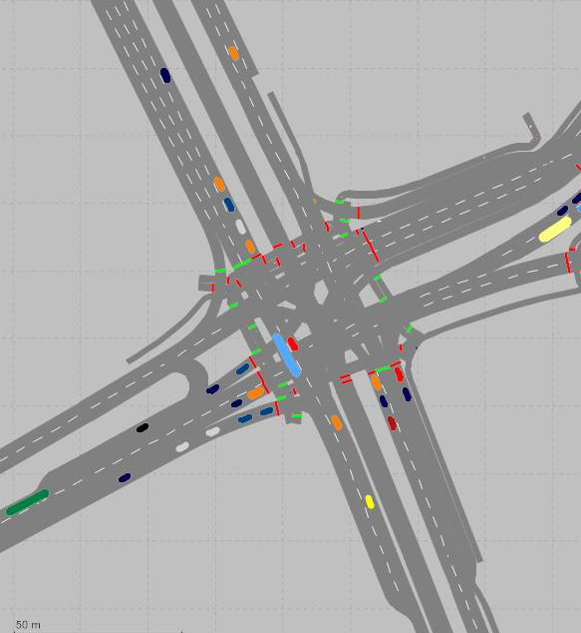
\includegraphics[scale=0.3]{VissimNet} \\
\textbf{ruch drogowy}, to położenie wszystkich pojazdów przez cały okres zapisu:  \\
$\lbrace x_{\alpha}(t): t \in T, a \in A \rbrace$  
\end{center}
\end{frame}

\label{2.4}
\begin{frame}{Reprezentacja ruchu}{trajektorie}
\begin{columns}
\column{0.2\textwidth}
położenie pojazdu w czasie
\column{0.8\textwidth}
\includegraphics[scale=0.55]{trajektorie1}
\end{columns}
\end{frame}

%\begin{frame}{Reprezentacja ruchu}{mikroskopowy pomiar pojazdu}
%\begin{center}
%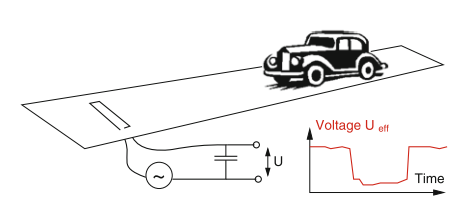
\includegraphics[scale=0.6]{petla}
%\end{center}
%pomiar stacjonarny (urządzenie mierzące stoi, pojazd jedzie) \\
%np. z pętli indukcyjnej
%\end{frame}

\label{2.5}
\begin{frame}{Reprezentacja ruchu}{mikroskopowy pomiar pojazdu}
\begin{center}
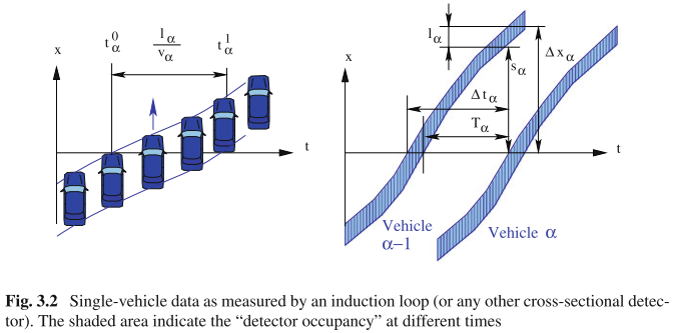
\includegraphics[scale=0.6]{petla2}
\end{center}
\begin{itemize}
\NumTabs{2}
\item \alert{długość pojazdu} \tab{$l_\alpha = v_\alpha (t^1_\alpha - t^0_\alpha)$}
\item \alert{odstęp czasowy} \tab{$\Delta t_\alpha = v_\alpha (t^0_{\alpha} - t^0_{\alpha-1})$}
\item \alert{odstęp podłużny} \tab{$d_\alpha = v_{\alpha-1}\Delta t_\alpha$}
\item \alert{prędkość}  \tab{dla pętli podwójnych}
\end{itemize}
\end{frame}

\label{2.6}
\begin{frame}{Reprezentacja ruchu}{gromadzenie danych z różnych źródeł}
\begin{columns}
\male
\column{0.3\textwidth}
wiele źródeł danych:
\begin{itemize}
\item pętle stacjonarne, 
\item pojazdy sondujące (FCD)
\item pomiar trajektorii na krótkim odcinku 
\item przelot helikopterem
\end{itemize}

\column{0.7\textwidth}
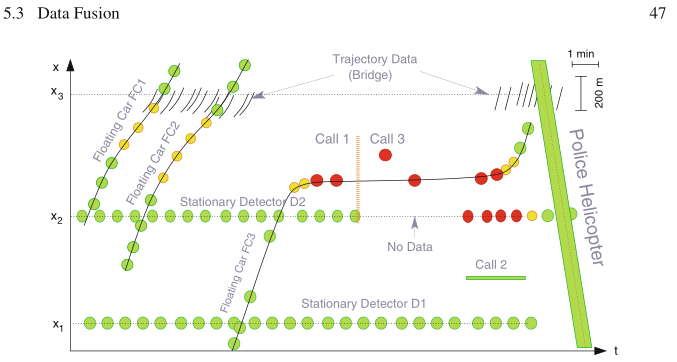
\includegraphics[scale=0.45]{Fusion}
\end{columns}
\end{frame}

\label{2.7}
\begin{frame}{Reprezentacja ruchu}{jak opisać to, co obserwujemy?}
\begin{enumerate}
\item model makroskopowy statyczny
\item model makroskopowy dynamiczny
\item modele mikroskopowe
\end{enumerate}

\end{frame}

\label{2.7}
\begin{frame}{Reprezentacja ruchu}{agregacja wartości mikroskopowych do opisu makroskopowego}
\begin{center}
\includegraphics[scale=0.3]{trajektorie1}
\end{center}
\NumTabs{2}
liczba pojazdów \tab $N$ \\
potok \tab $Q(x,t) = \Delta N / \Delta t$ \\
średnia prędkość  \tab $V(x,t) = \langle v_\alpha \rangle $ \\
gęstość  \tab $ \rho (x,t) = \frac{Q(x,t)}{V(x,t)}$
\end{frame}

\begin{frame}{Funkcja oporu}{statyczny makroskopowy opis ruchu}
\begin{center}
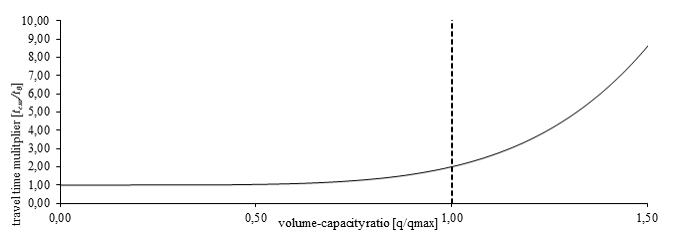
\includegraphics[scale=0.4]{VDF}
\end{center}
\begin{itemize}
\item w modelowaniu strategicznym (planistyka) pomijamy zmienną czasu $q_a(t)\rightarrow q_a$
\item czas przejazdu jest szacowany $t$ jako funkcja wykorzystania przepustowości $q/q_{max}$ 
\male \begin{equation*}
t = t_0 \cdot \left( 1+ a \cdot \left( \frac{q}{q_{max} }\right)^b \right)
\end{equation*}
\normalne
\item nie ma tu nigdzie indeksu czasu, cały opis stanu korzysta ze zmiennych zagregowanych \\ $Q_a = \Delta N  /  \Delta T$ , $\Delta T$ = 1h
\end{itemize}
\end{frame}

\begin{frame}{Funkcja oporu}{statyczny makroskopowy opis ruchu}
\begin{center}
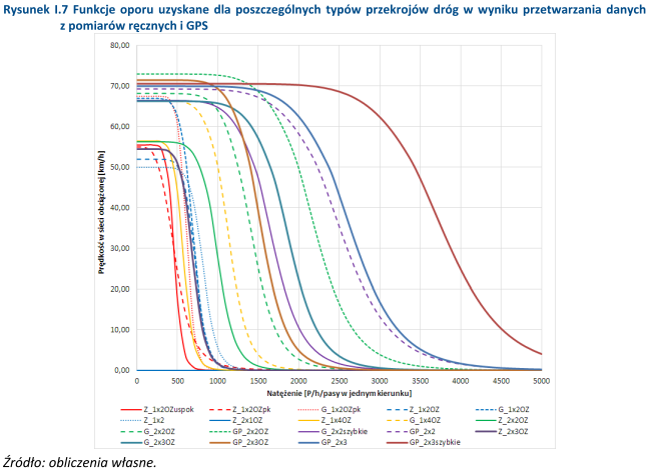
\includegraphics[scale=0.5]{VDF_WBR}
\end{center}
\male WBR 2015
\end{frame}

\begin{frame}{Markoskopowa statyczna funkcja oporu}{problem}
\begin{columns}
\column{0.3\textwidth}
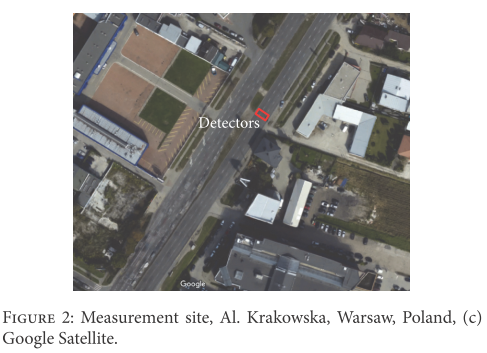
\includegraphics[scale=0.3]{WWA}
\column{0.7\textwidth}
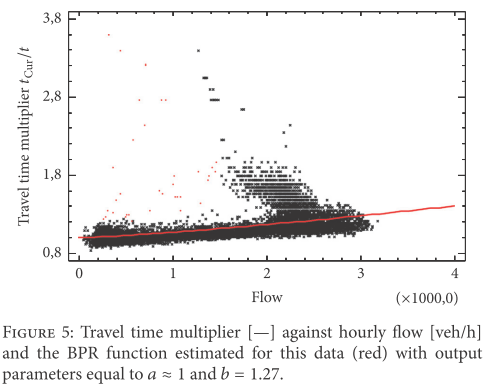
\includegraphics[scale=0.5]{VDF_problem}
\end{columns}
.\\zależność funkcyjna między potokiem, a prędkością\\ \textbf{nie zachodzi}
\end{frame}

\begin{frame}{Diagram fundamentalny}{}
trzy makroskopowe zmienne opisu ruchu:
\begin{itemize}
\item potok $Q$ [poj./h]
\item prędkość $v$ [km/h]
\item gęstość $k$ [poj./km]
\end{itemize}
podstawowa zależność hydrodynamiczna:
\begin{itemize}
\item $Q=kv$,\item $v=Q/k$,\item$k=Q/v$ 
\end{itemize}
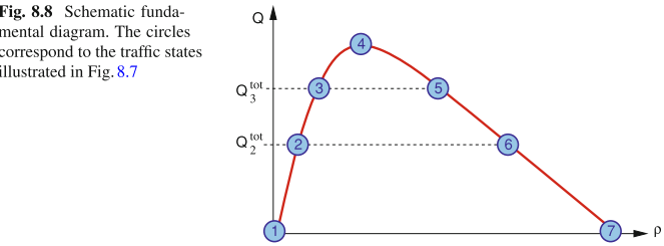
\includegraphics[scale=0.4]{diagram}
\end{frame}

\begin{frame}{Diagram fundamentalny}{}
\includegraphics[scale=0.45]{funddiag}
\end{frame}

\begin{frame}{Diagram fundamentalny}{rozszerzenie z opisu punktowego na przestrzeń i czas}
\alert{Diagram} opisuje stan w danej chwili czasu $t$ w danym miejscu $x$: \\
$k(x,t)$,  $q(x,t)$, $v(x,t)$.
\\ jak określić dynamikę w czasie: $\frac{dk}{dt}$ i w przestrzeni $\frac{dk}{dx}$ ?
\\ \alert{Fala wzburzeniowa}
\end{frame}

\begin{frame}{Diagram fundamentalny}{fala wzburzeniowa}
\includegraphics[scale=0.4]{diagpl}
\begin{equation*}
w(x,t)=\frac{dq(x,t)}{dk(x,t)}
\end{equation*}
\textbf{fala} - pochodna diagramu fundamentalnego \\
kierunek i prędkość propagacji zmiany stanu (gestości)
\end{frame}

\begin{frame}{Wykres czasoprzestrzenny}{rekonstrukcja}
\begin{columns}
\column{0.4\textwidth}
\includegraphics[scale=0.2]{falediag}
\column{0.6\textwidth}
\includegraphics[scale=0.25]{spacetime}
\end{columns}
\male
kolor oznacza prędkość (im ciemniej, tym mniejsza prędkość $v$ \\
dla każdego punktu na diagramie mozemy odczytać prędkość $q/k$ , \\ 
prędkość i kierunek fali $w$\\
i odtworzyć ruch w czasie (oś $x$) i w przestrzeni (na odcinku, oś $y$)
\end{frame}

\begin{frame}{Wykres czasoprzestrzenny}{przykład}
\includegraphics[scale=0.4]{spacetime2}
\bmale
\begin{itemize}
\item zator i spowolnienie od godziny 7 do 9 na 472 kilometrze
\item zator z 482 kilometra propaguje \textbf{wstecz} i dociera (przed dziesiątą) na 466 kilometr
\item wjeżdzając na odcinek o godzinie 9 trafimy na kilka różnych korków 'stop-and-go wave'
\end{itemize}
\end{frame}

\begin{frame}{Dynamiczny makroskopowy model przepływu}{synteza}
Dynamiczny makroskopowy model przepływu:
\begin{itemize}
\item wyniki jako funkcja czasu i przestrzeni $q(x,t)$
\item uproszczony graf
\item nie ma pojedynczych pojazdów, a \textbf{potoki}
\item model deterministyczny, tzn. wszyscy zachowują się tak samo - przeciętnie
\item bardzo szybki w obliczeniach (do zastosowań w czasie rzeczywistym)
\item bogata reprezentacja zjawiska
\end{itemize}
\end{frame}

\begin{frame}{Dynamiczny makroskopowy model przepływu}{przykład wyników}
\includegraphics[scale=0.4]{tre1}\\
\includegraphics[scale=0.4]{tre2}
\end{frame}

\begin{frame}{Model mikroskopowy}{podsumowanie}
Model mikroskopowy:
\begin{itemize}
\item wyniki jako trajektorie indywidualnych pojazdów $x_\alpha(t)$
\item rozbudowany graf (uwzględnia geometrię i inżynierię ruchu)
\item model stochastyczny, losowy (to dobrze, a nawet źle) 
\item długi czas obliczeń 
\item do analiz konieczność agregacji i uśredniania z kilku symulacji
\end{itemize}
\end{frame}


\begin{frame}{Powtórzenie}
\begin{center}
\includegraphics[scale=0.45]{przykladspacetime}

\male 
Pytania:
\begin{itemize}
\item co oznacza pozioma czarna linia?
\item jaki jest czas przejazdu i opóźnienie dla pogrubionego pojazdu?
\item jaki jest dopływ pojazdów/h dla $t\leq 20$ (poj./h)?
\item jaka jest prędkość w ruchu swobodnym (km/h)?
\item jaka jest gęstość pojazdów w kolejce (poj./km)?
\item jaki jest przepływ pojazdów po usunięciu przeszkody (poj./h)?
\item jaka jest prędkość fal: budowania i rozładowywania się kolejki (km/h)?
\end{itemize}
\end{center}
\end{frame}


\subsection{Podsumowanie}
\begin{frame}{Dziękuję za uwagę}{zapraszam do dyskusji}
na następnym wykładzie:
\begin{itemize}
\item model mikroskopowy deterministyczny (Newell's car-following model)
\item model mikroskopowy rozbudowany (Wiedeman)
\item modele wyboru dyskretnego
\begin{itemize}
\item zmiana pasa 
\item włączenie się do ruchu
\end{itemize}
\end{itemize}
\end{frame}

\begin{frame}{Dziękuję za uwagę}{zapraszam do dyskusji}

\bmale źródła wszystkich obrazów (jeśli nie podano inaczej) \\ M. Treiber, A. Kesting Traffic Flow Dynamics, Spirnger 2013, lub własne
\end{frame}

\end{document}
